\hypertarget{Fundamentals of Overlapped Sounds}{%
\chapter{Fundamentals of Overlapped Sounds}\label{cha:fundamentals}}

In this thesis, the core part is focussed on \emph{analysis} and \emph{processing} of sound recordings of music and speech, commonly referred to as \emph{audio signals}.
In this chapter, we therefore introduce basic concepts of digital audio signals which are relevant to apprehend the remaining chapters.

\hypertarget{Audio Signals}{%
\section{Audio Signals}\label{sec:specifics-of-audio-signals}}

When a sound wave travels through a medium like air, a signal can be captured using a microphone by measuring the local pressure deviation over time.
Such a signal can be written as a function \(x(t)\), continuous in both time \(t \in \sR\) and the amplitude \(x(t) \in \sR\).
An \emph{audio signal} is meant to be perceived by the human auditory system --- through our ears.
Therefore, we can observe specific properties, consistent with the limitations of the human hearing system, for example in dynamics as well as a limited signal bandwidth.
Many other signals exist with similar characteristics such as signals from finance, geophysics, meteorology or medical data.
The result is that audio research is inspired by applications of other fields of signal processing and vice versa.

\hypertarget{digital-representations-of-audio-signals}{%
\subsection{Digital Representations of Audio
Signals}\label{digital-representations-of-audio-signals}}

Today, digital representations are used to store, analyze or process audio signals conveniently.
A digital audio signal can be obtained from an analog signal using analog-to-digital/digital-to-analog converters (ADC/DAC) which can be found in almost any every-day device such as laptops and smartphones.
In short, this process includes two steps: first, the continuous time signal \(x(t)\) is converted to a discrete time series, so that one sample\footnote{Please note, that the use of the word \emph{sample} will have different meanings in the context of machine learning, where a sample is an instance of a full signal instead of a single time step.} \(x_n\) is \emph{sampled} with equidistant steps \(T\); second, the amplitude values are \emph{quantized} resulting in a vector \(\vx \in \sZ\), represented as a one dimensional time series of amplitudes.
An important parameter in the process of digitization is the sample rate \(F_s = 1/T\) where \(T\) is the sampling period.
% Often, \(F_s\) has a significant effect on the quality of audio signals.
% And, it is the objective of a real-world audio system not to introduce perceivable degradation in audio quality when a digital signal is reproduced over headphones or loudspeakers.
% Due to the Nyquist-Shannon sampling theorem, the sample rate needs to be at least twice the bandwidth of the analog signal.
To facilitate the full human hearing range of 20~\si{\hertz} - 20~\si{\kilo\hertz}~\cite{fastl90, moore89}, due to the Nyquist-Shannon sampling theorem, often, sample rates of at least 40~\si{\kilo\hertz} are chose.
However, for many applications, a lower sampling rate is sufficient, e.g., in speech communication where intelligibility often is more important than quality.
For further details, we refer the reader to audio signal processing basics such as~Chapter 1 in~\cite{proakis96} or Chapter 2 in~\cite{Mueller15}.

\hypertarget{time-frequency-representation}{%
\subsection{Time-Frequency Representation}\label{sub:time-frequency-representation}}

We often analyze sounds in the frequency domain where the reduced redundancy of the signal improves the computational efficiency of signal processing methods, especially for speech and music that have periodicities.
It is common to achieve this through the use of discrete Fourier transform (DFT) and its fast FFT implementation~\cite{cooley65} (for details, the reader is referred to~Chapter 4 of~\cite{proakis96}).
Spectral representations also relate to our human auditory system~\cite{zwicker13, moore89}, allowing us to process sounds closer to how we perceive them.
\par
The periodicity of real-world sounds, usually only holds for short durations of several milliseconds, often referred to as ``quasi-stationarity''.
We analyze and process short-time spectra, computed in an overlapped fashion, resulting in a \emph{time-frequency} (TF) representation.
The short-time Fourier transform (STFT) is the most commonly used TF representation~\cite{mcaulay86}.
It encodes the time-varying spectra into a matrix \(\mX\) with frequencies \(k\) and time frames \(n\).
\par
STFT matrices \(\mX \in \sC^{n \times k}\) are complex and include phase information.
When sounds are processed in the time-frequency domain, the transformation greatly benefits from being invertible to reconstruct a time domain signal.
However, analysis and processing is often focussed  on the \emph{magnitude} \(|\mX|\) or the \emph{spectrogram} \(|\mX|^2\).

\subsection{Fundamental Frequency and Harmonicity}

\begin{figure}[h!]
  \centering
  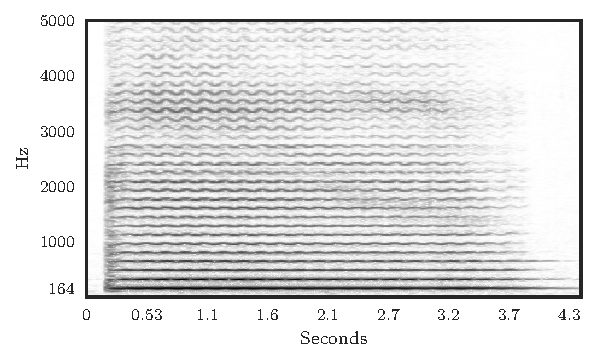
\includegraphics[width=0.8\columnwidth]{gfx/cello.pdf}
  \caption{Spectrogram of single violoncello note (E3) of a fundamental frequency \(F0\) of about 164\si{\hertz}. The vibrato is clearly visible in the upper part of the harmonic spectrum. The audio signal is part of the MUSERC dataset~\cite{stoeter15acm}.}%
  \label{fig:cello_example}%
\end{figure}

Speech and music signals are characterized by its periodicity.
And it is this property we perceive as \emph{pitched}.
\emph{Pitch} is defined by Klapuri in~\cite{klapuri06book} as 

\begin{quote}
``a perceptual attribute which allows the ordering of sounds on a frequency-related scale extending from low to high.''
\end{quote}

It is important to note that \emph{pitch} is a subjective measure.
The objective equivalent is referred to as the \emph{fundamental frequency} (\(F_0\))\footnote{Pitch and $F_{0}$ are often used synonymously in audio research. 
Even though this is incorrect, we sometimes may refer to other work where pitch instead of $F_{0}$ is used.}.
An example of a harmonic signal can be seen in Figure~\ref{fig:cello_example} that depicts a single note (E3) played by violoncello.
\(F_{0}\) can be defined as the lowest frequency/partial of a harmonic signal.
All frequencies together formed by the integer multiples of the fundamental frequency are named \textit{harmonics}~\cite{schenker54}.
When the fundamental frequency changes, the frequencies of these harmonics change accordingly.
This results in the typical comb-like structure of harmonic signals when analyzed in the time-frequency domain.
For a a detailed overview into the research field of pitch and \(F_{0}\), the reader is referred to~\cite{klapuri06book}.

\subsection{Time-Variant Audio Signals}\label{sub:time-variant-audio-signals}

Audio signals are considered to be stationary or time-invariant when their properties such as the amplitude of the fundamental frequency of the signal do not change over time.
% A stationary sound can turn into time-invariant sound using modulations
The signal becomes time-variant when an external function changes (modulates) the parameters of a signal over time.
These simple idea were the basis for many break-through inventions such as radio transmission~\cite{shannon48}.
In the case of audio signals, often both the modulating function (modulator or carrier) and the signal being modulated (input) are periodic.
Signal modulations are often created intentionally but also occur naturally in many real-world audio signals such as speech.
In the following, we will present audio modulation categories and their cause, underlining the importance of them.

\subsubsection*{Audio Signal Communication}

% The transmission of an audio signal using a modulator/demodulator (modem) system may be one of the most essential applications for audio modulations. 
% The principle is used the broadcasting of radio using a high-frequency carrier signal that is modulated by an audio signal to be transmitted, which is assumed to be of lower frequency than the carrier signal.
% The modulator is targeted to vary the amplitude or the frequency of the carrier signal.
If we imagine a sinusoidal carrier signal $x(t) = \cos \omega_c t$, \emph{amplitude modulation} (AM) is applying by a modulation function $a(t)$ so that:

% We assume that we can separate overlapping partials of the sources based on differences in amplitude and/or frequency modulation, resulting in the following model for a signal with $P$ commonly modulated partials
% \begin{equation}
%   \begin{array}{l}
%    x(n) = \displaystyle \sum_{p=1}^{P} \Big[\big(1 + a(n)\big) \\
%    \hspace{3.5em}\displaystyle \cdot\sin \Big(2\pwe f_{p,0}\big(n + \frac{1}{f_{1,0}} \sum_{m=m_0}^{n}{f(m)} \big) + \phi_{p,0} \Big)\Big] ,
%   \end{array}
% \end{equation}
% where effectively the amplitude modulation is $a(n)$ and the frequency modulation of the first partial is $f(n)$.

\begin{equation*}
    s_{AM}(t) = a(t) \cos \left( \omega_{c} t\right).    
\end{equation*}

In comparison to AM, Frequency modulation (FM) varies the frequency of the carrier, so that:

\begin{equation*}
    s_{FM}(t) = A e^{j\left(\omega_{0} t + m \sin \left(\omega_ { m } t \right)\right)}
\end{equation*}

where A is the amplitude, $\omega_0$ is the carrier frequency, $\omega_m(\theta)$ is the instantaneous modulation frequency, and $m$ is the modulation index $m = \frac{\Delta \omega_0} { \omega_{m} }$.

The Fourier spectrum of $s_FM(t)$, which depends, in theory, on Bessel functions that do not admit a closed-form expression, is intractable in practice~\cite{abramowitz64}.
% For applications where the modulation frequencies are a lot smaller than the carrier frequency, the spectrum that results by frequency modulations is similar to those of amplitude modulations.
% This is the reason why algorithms that aim to capture the amplitude modulation will also observe frequency modulations.
% The total bandwidth in this scenario is approximately $2\Delta \omega_0$, as found by Carson in~\cite{carson22}.\par
For audio communication such as FM radio, the modulation frequency or rate is the same as the audio signal being transmitted (audio rate modulations).
In music signals, the carrier could be a single note, played by a violin and the modulation signal is the movement of the finger on the fretboard, producing a vibrato effect.
In music or speech, these modulations are much slower --- typically up to 10~\si{\hertz} (slow) or up to 100~\si{\hertz} (medium/fast).

\subsubsection*{Modulations in Music --- Vibrato}

Both, frequency and amplitude modulations are a recurrent phenomenon in music as well.
In traditional instruments, modulations are known to as \emph{vibrato}, defined by~\cite{seashore31} as

\begin{quote}
``...a periodic pulsation, generally involving pitch, intensity, and timbre, which produces a pleasing flexibility, mellowness and richness of tone.''
\end{quote}

Pitch and intensity vibrato can directly be mapped to AM and FM, a timbre vibrato, however, is not easily defined and describes a joint AM/FM modulation~\cite{desain99}.
Vibrato is an essential playing style for string instruments like a violin. 
For these instruments, that are usually plucked or bowed, the strings are the primary source of excitation that is modulated in frequency by the player's finger on a fretboard~\cite{macleod06}.
Modulations are also present in woodwind and brass instruments; however, instead of the excitation signal, the modulations affect the resonator.
Many musicians use similar modulation rates to perform a vibrato.
They vary across musicians and is usually in the range of 4-8\si{\hertz}.
A detailed overview of the different musical instruments and their modulation characteristics are presented in~\cite{fletcher01}.
\par
Real instruments are not capable of purely amplitude modulated sounds (\emph{tremolo}). 
Today, many instruments are electric or are attached to electronic effects where such modulations can be applied using digital or analog signal processing.
For example, popular electric pianos like the ``Fender Rhodes'' can include an optional tremolo effect\footnote{Even though it is labeled as \emph{vibrato}.}.
In its most pure form, synthesizers like~\cite{pinch09, buchla05} allow modulating almost any parameters of a sound using low-frequency oscillators (LFOs) or envelopes that produce sinusoidal, square or triangle functions of any rate.
One of the most important sound synthesis methods --- FM Synthesis --- became popular in the early days of digital signal processing. 
Chowning~\cite{chowning73} found that the modulation of sinusoids using audio rate modulators provides a computationally efficient way of producing fairly complex sounds which mimic, e.g. piano sounds using just four sinusoidal modulators.
\par
It turns out that instrumental vibrato has similar properties compared to vibrato produced in singing voice.
Vocal vibrato mainly dependents on frequency modulation even though amplitude fluctuations are present~\cite{sundberg94}. 
The vibrato rate is similar to that of instrumental vibrato with its peak around 5~\si{\hertz}.

\subsubsection*{Modulations in Speech}

Unlike singing voice, speech modulations are part of human communication and therefore part of our language.
Modulations in speech include medium to fast modulations of up to a few hundred Hertz, perceived as \emph{roughness} or \emph{residue pitch}.
However, often research is focussed on slow modulations around 4~\si{\hertz}~\cite{greenberg97, fuellgrabe09} that correlate to the syllable rate~\cite{plomp83, houtgast85}.
In fact, it was found in~\cite{joris04} that speech is the reason why our human auditory system is so sensitive to amplitude modulations and even our brain in capable of processing rhythm-like envelope fluctuations of the same rate~\cite{schreiner88, plomp83}.

\subsubsection*{The importance of Slow Modulations}

% Table~\ref{tab:modulations} summarized the many types of modulations in audio signals.
It is interesting to observe that many modulations have a rate of around 5~\si{\hertz}. 
Zwicker found in~\cite{zwicker52} that humans are very sensitive at detecting amplitude modulations at such a low modulation frequency.
This observation can be confirmed when looking at physical modulations that occur when humans suffer from vocal tremor~\cite{ramig87} or Parkinson~\cite{botzel14}: in both cases, muscle contractions are actuated with the same frequency, indicating that these modulations are natural for humans.

% \begin{table}[]
% \scriptsize
% \centering
% \begin{adjustbox}{angle=90}
% \begin{tabular}{@{}lllp{3.5cm}ll@{}}
% \toprule
%                           & Carrier Signal    & Modulation Function & Modulated Parameters        & Modulation rate & References\\ 
% \midrule
% AM/FM/PM                  & HF Sinusoid       & any audio signal    & amplitude, frequency, phase & up to 20~\si{\kilo\hertz}     & \cite{shannon48}        \\
% String Vibrato & String Excitation & sinusoidal-like     & string length   & 5-7~\si{\hertz}          & \cite{fletcher01, macleod06}\\
% Woodwind and Brass Vibrato & Resonator & sinusoidal-like & amplitude, timbre               & 4-8~\si{\hertz}          & \cite{fletcher01, gilbert05}\\
% Modular Synthesizer       & any audio signal  & LFO                 & any parameter               & not limited     & \cite{buchla05, pinch09}\\ 
% Electronic Organ with Tremolo  & instrument sound & doppler effect      & amplitude and frequency & 1~\si{\hertz}/7~\si{\hertz} & \cite{leslie49} \\
% Singing Voice  & vocal &  sinusoidal/triangular &  amplitude and frequency & 5-8~\si{\hertz} & \cite{sundberg94} \\
% Speech  & glottal pulse, language & not defined & amplitude, frequency, \newline phoneme duration, timbre& 4-10~\si{\hertz} & \cite{plomp83, fuellgrabe09}\\
% Parkinsonian tremor  & muscle activity &  sinusoidal-like & amplitude & 5~\si{\hertz} & \cite{botzel14}\\
% Auditory cortex  & nerve activity &  sinusoidal-like & amplitude & up to 20~\si{\hertz} & \cite{schreiner88}\\
% \bottomrule
% \end{tabular}
% \end{adjustbox}
% \caption{Overview of modulations in audio signals and a selection of their respective properties.}%
% \label{tab:modulations}
% \end{table}

\hypertarget{sources-and-mixtures}{%
\section{Sources and Mixtures}\label{sources-and-mixtures}}

In the real world, single isolated audio signals are rare.
Instead, we are faced with sets of \emph{sound sources} that make up an \emph{acoustical sound scene}.
When multiple sources are active at the same time, the sound that reaches our ears or is recorded using a microphone is superimposed or \emph{mixed} to a single sound.
A \emph{mixture} represents a mapping from a set of sources \(\mathbf{s}\) to an output signal \(\mathbf{x}\).
There exist a variety of different mixing models that are utilized in literature.
\par
Usually these are build upon several assumptions to constrain the scenario and model specific aspects of real world signals.
The most important assumption is that the mixture is the linear sum of all sources.
Another differentiation is made between instantaneous or convolutive mixtures.
For instantaneous mixtures, all sources are mixed using fixed mixing parameters \(a_j\).
This is the typical scenario when sources are mixed using a mixing console (pan-pot mix).
In \emph{convolutive} mixtures, each source \(\mathbf{s_j}\) is convolved by a filter response \(r_j\) before summation.
\par
Usually, the mixing process is assumed to be time-invariant but for a variety of signals, such as live recordings with moving sources, it can also be time-variant.
The mathematical notations of different mixing models are summarized in Table~\ref{tab:mixing_models}.
\par
In the remainder of this thesis, we will only consider the linear case of time-invariant mixing, but many of the methods could be transferred to other cases.

\begin{table}[]
    \centering
\begin{longtable}[]{lll}
\toprule
\begin{minipage}[b]{0.26\columnwidth}\raggedright
\strut
\end{minipage} & \begin{minipage}[b]{0.32\columnwidth}\raggedright
Instantaneous\strut
\end{minipage} & \begin{minipage}[b]{0.3\columnwidth}\raggedright
Convolutive\strut
\end{minipage}\tabularnewline
\midrule
\endhead
\begin{minipage}[t]{0.26\columnwidth}\raggedright
Time-Invariant\strut
\end{minipage} & \begin{minipage}[t]{0.32\columnwidth}\raggedright
\(\mathbf{x}=\sum_{j=1}^{J}a_j\mathbf{s}_j\)\strut
\end{minipage} & \begin{minipage}[t]{0.3\columnwidth}\raggedright
\(\mathbf{x} = \sum_{j=1}^{J}r_{j} \ast \mathbf{s}_j\)\strut
\end{minipage}\tabularnewline
\begin{minipage}[t]{0.26\columnwidth}\raggedright
Time-Variant\strut
\end{minipage} & \begin{minipage}[t]{0.32\columnwidth}\raggedright
\(\mathbf{x}=\sum_{j=1}^{J}a_j(n)\mathbf{s}_j\)\strut
\end{minipage} & \begin{minipage}[t]{0.3\columnwidth}\raggedright
\(\mathbf{x} = \sum_{j=1}^{J}r_{j}(n) \ast \mathbf{s}_j\)\strut
\end{minipage}\tabularnewline
\bottomrule
\end{longtable}
    \caption{Overview of linear mixing models for a mixture \(\mathbf{x}\), sources \(\mathbf{s}_j\) and a filter response \(r_j\).}
    \label{tab:mixing_models}
\end{table}

\subsubsection*{Specifics of Music Mixtures}
\label{par:specifics_of_music_mixtures}

In music, the process of mixing is an essential step in the process of music creation.
Mixing sources are a creative task that involves recording engineers and tonmeisters, and often the artists itself.
In today's digital mastering processes, professionally produced music consists of several intermediate mixing steps before the final mixture is produced:

\begin{description}
  \item[1) Microphone Recording:] in this step, the analog sources are captured and D/A converted. 
  Vocals and other acoustic instruments are recorded using one or multiple microphones.
  Electric instruments such as electric guitars, keyboards or synthesizers may be amplified and then directly digitized.
  \item[2) Raw Source Image:] the digital raw source signals are grouped and mixed into a \emph{source image} (also \emph{stem}).
  This grouping involves a creative process; hence it is usually done by a recording engineer.
  The source image is mixed to a specific number of output channels (e.g., stereo) even though the recording may have used less (e.g., vocals) or more than two microphones (e.g., drums).
  In this stage, a panning is added to position the source images spatially.
  \item[3) Mastered Source Image:] for each of the images, an additional mastering step is be applied.
  At this stage, effects such as artificial reverberation are added.
  \item[4) Raw Mix:] the linear sum of all source images are mixed for the final output.
  \item[5: Mastered Mix:] again, an additional mastering is applied.
  Often, this step involves non-linear processing such as dynamic range compression.
\end{description}

This emphasizes that the definition of a source is subjective and depends on the application and its context. In this thesis, we mainly deal with tasks where we observe 4) and want to obtain 3) which is a common restriction made in tasks that are concerned with professionally produced music~\cite{sisec16}.

\hypertarget{processing-and-analysis-of-mixtures}{%
\section{Processing and Analysis of Mixtures}\label{sec:processing-and-analysis-of-mixtures}}

While in many ways, mixtures are not different to any other audio signal, two research questions stand out prominently:

\begin{itemize}
    \item Can we obtain \(\vs_j\) from \(\vx\)? 
    \item Can we find \(J\) from \(\vx\)?
\end{itemize}

These two questions are addressed in the scientific fields of \emph{sound source separation} and \emph{source count estimation}.

\subsection{Sound Source Separation}

One of the earliest work on audio source separation started in the mid 70s~\cite{miller73}.
Since then a large amount of contributions were made in this field, both, targeted at speech and music separation.
Due to this large number of contributions, it is hardly feasible to give an extensive overview on all existing methods in the context, and the reader is referred to~\cite{vincent18, comon10, rafii}.
\par
Source separation methods have relevant applications for music and speech mixtures such as attenuation of hearing aids, karaoke or music creation due to isolated sample composition.
It also indirectly helps for related task such as upmixing/remixing, improved music transcription or automatic speech recognition (ASR). 
\par
In the following, we present three ways to group separation scenarios:

\subsubsection*{Underdetermined vs. Overdetermined Separation}
As mentioned in Section~\ref{sources-and-mixtures}, generating sound mixtures is closely related to the process of mixing taken place during recording (speech) or with the help of professional recording engineers (music).
One assumption that was not mentioned before, is the importance of the number sensors or microphones used to create the mixture.
A source separation problem is \emph{over-determined} when the number of sources is smaller than the number of sensors; \emph{determined} when they are equal.
For these two cases, a large number of method exist and in a closed form solution is possible.
The reader is referred to~\cite{common10}, which is gives a detailed overview of these methods.\\
Many real world source separation problems, however, are under-determined and up to date for a large number of scenarios, the problem of separating sources is still very challenging.
\par
In this thesis we only focus on methods that perform separation on underdetermined mixtures.

\subsubsection*{Single Channel vs. Multichannel Separation}
% from zafar

Today music recordings are mostly produced for stereo output. 
In many music recordings certain assumptions can be made (and utilized) of how sources are balanced between the two stereo channels. 
E.g., often in popular music, a fixed panning for the vocals is correctly assumed.
\par
As a large number of recording nowadays is still stored as single channel, in this thesis we want to focus on this single channel separation only.

\subsubsection*{Blind vs. Supervised Separation}
A blind separation source separation system does not require additional information about the source signals, the location or acoustical environment to perform separation~\cite{makino07}.
In practice, blind source separation is ill-posed and it is not generally possible to find a single solution.
This why many proposed methods rely on additional information such as the acoustic environment, the musical score or the fundamental frequency~\cite{liutkus13, ewert14}.

\subsection{Vocal Accompaniment Separation}
The separation of music into two parts, the foreground lead (mostly the vocals) and the background accompaniment (drums, bass, other), is one of the most relevant scenarios in music separation with a large number of applications such as mixing karaoke or a capella tracks.
Vocal Accompaniment separation has specific issues and assumptions when compared to other separation scenarios like speech.
Many music separation methods often rely on knowledge about the mixing process as made in Table~\ref{tab:mixing_models}.
While there exist many source separation methods that aim to extract the actual raw audio recording (Step 1 in  Table~\ref{tab:mixing_models}), often it is sufficient to extract the source images from the raw mixture.
In a live recording, this results in inverting the process of convolution as well.
Separation of convoluted mixtures is a very active field in source separation described in~\cite{pedersen07}.
In the context of music a separation, however, this becomes less relevant as today's recording and studio mixing environment are mostly digital.
Here, the last step in creating music mixtures, as described earlier, is a linear mix.
While the source images can yield from a mixing process undergoing the various assumptions, for the case of a mixture of source images, we consider only linear mixing in this thesis.
For a more detailed description of this scenario and applications of source image extraction, see~\cite{sturmel12}.
\par
Another specific about music separation is that it is typically restricted to a well defined set of musical sources.
Often these restrictions need to be made because not for all kind of music separation scenarios, data sets are available.
Thus, the most popular task is to extract the vocals and the background of the music.
An extensive overview of music separation methods can be found in~\cite{rafii18}.
Even though the overview is focused on vocal accompaniment separation, most approaches can be generalized to other sources.
\par
To evaluate separation systems for this scenario, the majority of publications used the Blind Source Evaluation (BSS Eval) toolbox~\cite{fevotte05,vincent06} that provides ``different and complementary metrics for evaluating separation that measure the amount of distortion, artifacts, and interference in the results''~\cite{rafii18}.

\subsection{Estimating the Number of Sources}%
\label{sub:count_problemstatement}

\begin{figure}[ht!]
  \centering
  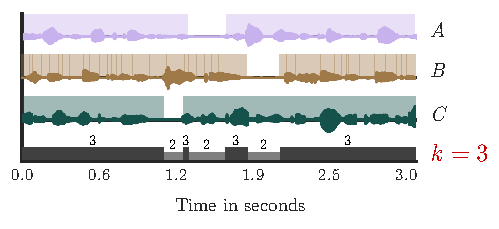
\includegraphics[width=0.8\columnwidth]{Chapters/08_Analysis_CountNet/figures/teaser.pdf}
  \caption{Illustration of three concurrent sources (A, B, C) and their respective activity. Bottom plot shows the mixture (input), the number of concurrently active sources and its maximum \(k\).}%
  \label{fig:teaser}%
\end{figure}

The number of sources is a simple but yet important information to be used in source separation and many other related research fields.
In real world applications, information about the actual number of concurrent speakers is often not available.
\par
The \emph{number of sources} \( \cardinality \in \mathbb{Z}^{+}_{0} \) appears to be a clearly defined property of a mixture. 
However the meaning of it can differ, depending on its application.
Let us assume that we have \(L\) sources and mixture of duration \(N\).
Further, we imagine a latent binary \textit{source activity} variable~$v_{nl}\in \left\{ 0,1 \right\}$ that indicates the activity of each source \(l\) and for each time instance \(n\).
Now, concerning the number of sources, two definitions of \(k\) can be imagined:

\begin{description}
\item[A)] maximum number of sources, even if not concurrently active. It is simply the sum of all sources that are active at least once within \(N\). This definition is more useful when the sources can be identified or detected first. This definition can also be considered as ``counting by detection''.
\item[B)] maximum number of concurrent speakers even if the sources belong to the same class. Here, it represents the maximum the mixtures concurrency. This definition is more useful as a preprocessing for a separation system since such a system would only require the number of \texttt{auditory\ streams} and not the number of (non-concurrent) sources. For such approaches it becomes possible to apply separation only when its ``needed''. This definition can also be considered as ``direct count estimation''\footnote{Please note the subtle difference between ``counting'', which refers to a sequential process and ``count estimation'' or ``denumerating'', which directly relate to an integer.}.
\end{description}

At short time scales A) is equal to B) because the sources/instrumentation usually does not change. 
In Fig.~\ref{fig:teaser}, we illustrate a setup featuring~$L=3$ unique sources.
At any given time, one can see --- given definition B) --- that at most~$k=L=3$ sources are active at the same time and~$k=2$ could be the outcome if a smaller excerpt would be evaluated.
In this thesis, we will pick definition B when concerned about developing methods to estimate the number of sources.
% However, when dealing with the human ability to estimate the number of sources, such a clear definition cannot be made.
% For instance, obtaining this number is even more challenging because the definition of a musical source cannot be given.
% In some scenarios, like popular western music, the sources to be separated, are grouped clear melody, bass, drums and ``other'' (the remainder), in other scenarios, e.g., the ``drums'' would count as multiple instruments.



